\documentclass{article}

\usepackage[utf8]{inputenc}
\usepackage{enumerate}
\usepackage{amsmath}
\usepackage{graphicx}
\usepackage{apacite}
\usepackage{blindtext}

\usepackage[margin=1cm]{caption}

\setlength{\parindent}{0.0in}
\setlength{\parskip}{0.1in}


\title{TDT4171 Artificial Intelligence Methods\\ Exercise 3}
\author{Edgar Vedvik -- edgarmv@stud.ntnu.no}
\date{2017-03-03}


\begin{document}
\maketitle


\section*{Introduction}
    In this exercise we were tasked with creating a decision support system for
    a decision problem of our own choice. The exercise listed some examples,
    and one of the examples was exactly a problem I was facing this week:
    \emph{Should I go out on Friday or stay home doing this exercise?} Next week
    I had many exercises that were due. I also had plans to go to an event
    Saturday evening. Therefore, I had good reason to stay home. However, as
    we all know, staying home Friday night doing exercises, while all your
    friends are out, isn't much fun.
    
    The exercise required that we had to measure the success of our choice. I
    measured this as the quality of life I would achieve when making this
    choice. The exercise also required that this decision problem had to
    contain at least 10 variables, and that half of them would have to be
    uncertain at the time the decision was made.

    The decision problem was modelled in GeNIe, which is a graphical user
    interface for solving just such a problem. GeNIe's interface was relatively
    easy to work with once I learned how to create nodes and connect them
    together and adding probabilities.

\section*{Model}

    Once I had chosen what decision problem to model, and my utility function.
    I followed the steps recommended in \citeA[pp. 634]{artificial} to create
    the model. The first step was to create a causal model. This meant making a
    dependency graph, with lines between each dependency. I identified the
    following variables as directly affecting my quality of life:
    \begin{itemize}
        \item Will I finish the exercise in time?
        \item Did I have a good time Friday night?
        \item The amount of money I have.
        \item My physical state (hungover / tired / well rested)
    \end{itemize}

    All of these variables are influenced by many other variables. Including
    all the variables is not in the scope of this report, but I have
    included those I found most important:

    \begin{itemize}
        \item Exercise deadline.
        \item How much of the exercise have i already done (progress).
        \item Are my friends going out on Friday?
        \item Did I work this week?
        \item Did I go out on Thursday?
        \item Do I have plans on Saturday?
        \item Will I make those plans?
    \end{itemize}

    \begin{figure}[ht]
        \centering
        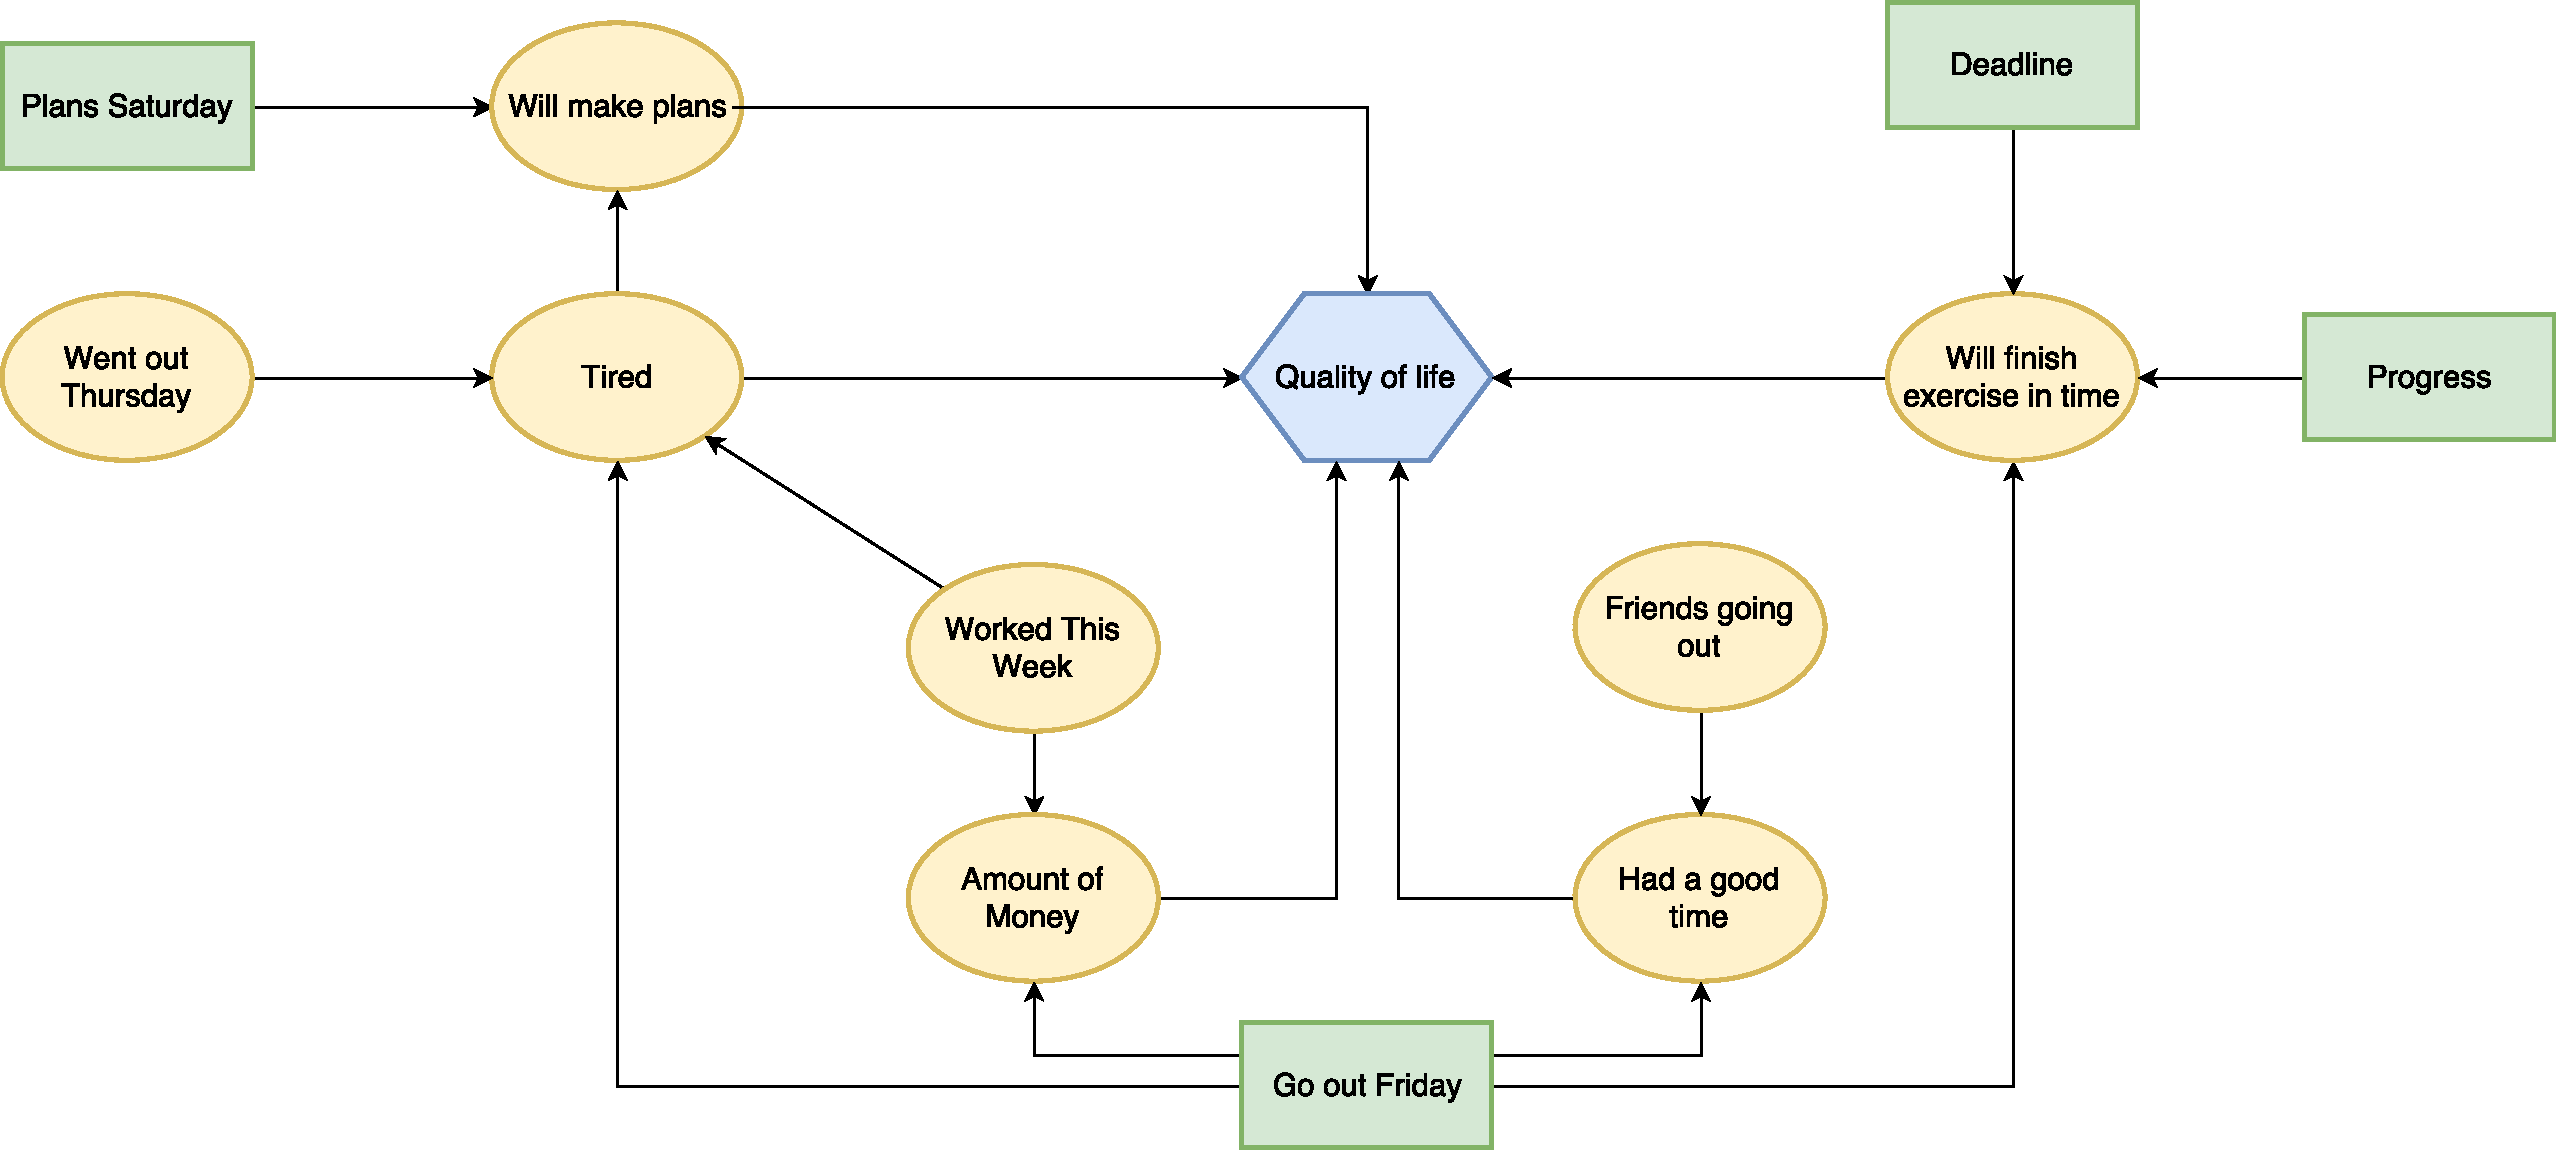
\includegraphics[width=\linewidth]{drawing.pdf}
        \caption{The model of the decision problem. The green rectangles are
        observable variables.  The yellow ellipses are unknown at the time
        the decision is made, and the blue hexagon is the utility.}
    \label{fig:model} \end{figure}

    After adding all the variables and identifying the dependencies between
    them I ended up with the model seen in Figure \ref{fig:model}. The majority
    of the dependencies are self-explanatory. Such as why \emph{Will finish
    exercise on time} depends on when the deadline is and how much of the
    exercise I have already done. One might think that it should also depend on
    whether I worked this week as well, since that would take time away from
    doing exercises. The reason why this is not the case is because when I
    work, I work mondays. and therefore it becomes too long ago for it to
    matter. If the exercise is due next week then it will be affected by work
    that week, but not this week. 


    The second step was to simplify and remove variables that did not affect the
    decision. Because my model was so simple and all variables affected my
    utility function, I skipped this step.

    Next step was to assign probability to each unknown state. Some of these
    were simple, like whether my friends are going out, if I have to
    work this week and the probability of going out on a Thursday. None of
    these variables depended on other variables, making figuring out the
    probability as easy as just remembering how often these things happen.

    With all the edge variables and decisions added, the more complex variables
    had to be created. These are also based mostly on empirical evidence. The
    most complex probability table was the \emph{Will finish exercise in time},
    which depended on when the deadline was, my progress on the exercise and
    whether I would go out on Friday. Since both deadline and progress had
    three values to choose from, making it a 18x2 big probability table. A
    small piece of it can be seen in Table \ref{tab:prob}.

    \begin{table}[ht]
        \centering
        \begin{tabular}{| c | c | c | c |}\hline
            Progress & \multicolumn{3}{|c|}{Halfway}\\ \hline

            Go out on Friday & \multicolumn{3}{|c|}{No} \\ \hline

            Deadline & Two weeks & Next week & Tomorrow\\ \hline

            Yes & 0.95 & 0.95 & 0.9\\ \hline

            No & 0.05 & 0.05 & 0.1\\ \hline
        \end{tabular}
        \caption{Probability of finishing the exercise before deadline.}
        \label{tab:prob}
    \end{table}

    Whether the deadline is next week or the week after, almost doesn't matter.
    I normally don't start exercises weeks ahead of time, so for me not to make
    it in time, depends on other factors that I have not added to my model
    (such as sickness). If the exercise was due on Monday, for example, then
    there should be a difference, but since I am already half way done, I
    should have more than enough time. We also see that even if the exercise
    was due tomorrow, the probability of making it is still very high. This is
    because I have no problem pulling an all-nighter if I have to. 

    The next step was to assign utilities. I decided to use an additive utility
    model because it seemed natural for this problem. My quality of life is
    improved more by finishing the exercise than being well rested for example.
    The value of each variable affecting my quality of life can be seen in
    Table \ref{tab:utility}. All of these are taken from my personal experience
    of what I value most in life. I decided that each value should be in the
    range $\left[ -10, 10 \right]$.

    \begin{table}[ht]
        \centering
        \begin{tabular}{| c | c |}\hline
            Variable &  Utility\\\hline
            Finish exercise & 9\\ \hline
            Tired & -1\\ \hline
            Made plans & 5\\ \hline
            Money(Broke, Some, Rich) & -1, 4, 6\\\hline
            Had a good time & 6\\\hline
        \end{tabular}
        \caption{How much the variables affect my quality of life.}
        \label{tab:utility}
    \end{table}
    
    I decided that my utility function should be the change in my quality of
    life. Meaning that it could be both negative and positive. My utility
    function therefore adds the inverse value for the inverse variable. For
    example, not finishing the exercise would add minus nine to the utility
    function. This does not apply to the money variable, since it is not a
    yes/no variable. With this, the best achievable quality of life is 27 and
    the worst is -22.

    \citeA[pp. 634]{artificial} suggests two more steps: verify and refine the
    model and perform sensitivity analysis. These two steps were done in
    parallel with the previous steps. Whenever a variable got a value that
    did not match with my perception of it, I went back and adjusted the
    probabilities.



\section*{Results}
    After following all the steps, I ended up with the model seen in Figure
    \ref{fig:genie}. I have entered evidence such as when the exercise is due
    and how much of it I had done. I also had plans Saturday so I entered that
    as well. The difference in staying home, doing exercise and going out are
    not that big, with only a difference in 1.5 between them. Regardless of my
    choice, my quality of life would improve,

    \begin{figure}[ht]
        \centering
        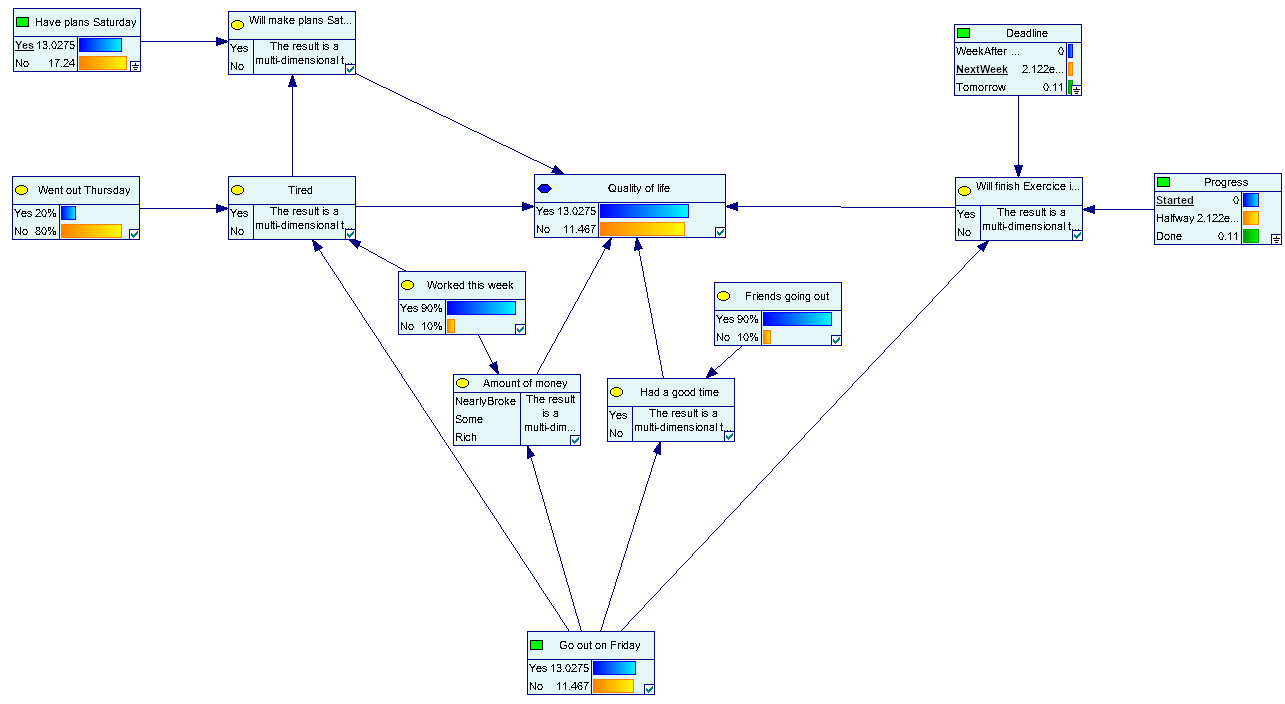
\includegraphics[width=\linewidth]{genie.png}
        \caption{The finished model in GeNIe.}
        \label{fig:genie}
    \end{figure}

    To make sure my model was good, I tried out a few other scenarios. The
    results can be seen in Table \ref{tab:tomorrow} and Table
    \ref{tab:saturday}.

    \begin{table}[ht]
        \centering
        \begin{tabular}{| c | c |}\hline
            & Quality of life\\\hline
            Went out & -0.4725\\\hline
            Did exercise & 6.067\\\hline
        \end{tabular}
        \caption{If the exercise was due Saturday instead of next week.}
        \label{tab:tomorrow}
    \end{table}

    If the exercise is due tomorrow, quality of life drops significantly
    regardless of my choice, but drops much more if I go out. It also matters
    very little whether the exercise is due next week or the week after, which
    is as expected since I usually don't do exercises that are due more than a
    week from now.

    \begin{table}[ht]
        \centering
        \begin{tabular}{| c | c |}\hline
            & Quality of life\\\hline
            Went out & 17.38\\\hline
            Did exercise & 12.59\\\hline
        \end{tabular}
        \caption{If I have no plans of going out on Saturday.}
        \label{tab:saturday}
    \end{table}

    If I do not plan on going out on Saturday, going out on Friday increases
    by about 4. This makes sense since I usually go out on at least Friday or
    Saturday. There is also a slight increase in staying home if I have no plan
    on Saturday. This points to that my model is not perfect, since ideally
    this should stay the same, or go down slightly.

\section*{Discussion}
    Overall, the results from my model matches my expectations. My quality of
    life increases regardless of my choice, since either I get to have fun or I
    am one exercise closer to being done for this semester. Both of which
    affects my life in a positive way. 

    There were, however, some inconsistencies. If I did not have plans on
    Saturday I expected the model to show a slight decrease in life quality if
    I then chose to not go out on Friday. However, my model gave it a slight
    increase. This is because, in my model, the quality of life is not
    dependent on a \emph{did I go out this weekend} variable, which it should
    have been.


\bibliography{references}
\bibliographystyle{apacite}

\end{document}
